\chapter{消化系统疾病}

\chapterabstract{本章主要介绍消化系统常见疾病(胃炎、消化性溃疡、病毒性肝炎、门脉性肝硬化、食管癌、胃癌、大肠癌及肝癌)的病理形态特点和临床病理联系,对这些常见疾病的病因及发病机制也进行了简单的介绍。要求学员重点掌握溃疡病的病理变化及并发症、消化系统四大恶性肿瘤肉眼及组织学类型、病毒性肝炎和门脉性肝硬化的基本病理变化;熟悉慢性胃炎的基本病理特点、早期食管癌、胃癌及肝癌的概念、各型肝炎的病变特点。了解这些常见疾病的病因、发病机制及临床病理联系。}

\begin{framed}
{案例8-1}

{【病例摘要】}

患者,男,67岁,因中上腹隐痛3个月余入院。既往体健。两个月来无明显诱因下出现中上腹隐痛不适,伴反酸,嗳气,伴食欲下降,近期伴体重下降。无恶心,呕吐,呕血,便血,黑便,无腹胀,腹泻,里急后重感。查胃镜示:胃角见一大小约3.0cm溃疡面,质地硬,触之易出血。

{【问题】}

(1)该患者胃部病变可能诊断有哪些?

(2)试分析其可能的生长扩散机制。
\end{framed}

\section{慢性胃炎}

胃炎是发生在胃黏膜的炎症,是十分常见的疾病。可分为急性胃炎(acute
gastritis)和慢性胃炎(chronic
gastritis)。急性胃炎包括急性刺激性胃炎、急性出血性胃炎、腐蚀性胃炎和急性感染性胃炎。

慢性胃炎是指由不同病因引起的胃黏膜的慢性非特异性炎症,发病率较高。慢性胃炎主要分为慢性浅表性胃炎(chronic
superficial gastritis)、慢性萎缩性胃炎(chronic atrophic
gastritis)、慢性肥厚性胃炎(chronic hypertrophic
gastritis)、疣状胃炎等几种类型。

\subsection{病因及发病机制}

慢性胃炎的病因尚未完全明了,可能与以下因素有关:

\subsubsection{感染因素}

近年来研究发现幽门螺杆菌({helicobacter pylori}
)的感染与慢性胃部疾患(胃炎、胃溃疡)及胃癌的发生密切相关。另外,口、鼻、咽喉部的慢性感染灶的细菌、毒素吞入胃内,对胃黏膜刺激亦可导致慢性炎症。

\subsubsection{长期服用刺激性食物或药物}

浓茶、烈酒、喜食过于辛辣、过于粗糙的食物及滥用水杨酸等药物对胃黏膜有损害。

\subsubsection{十二指肠反流}

十二指肠内胆汁反流至胃内,破坏胃黏膜屏障,可导致发病。

\subsubsection{自身免疫损伤}

部分慢性萎缩性胃炎患者血中的抗壁细胞抗体(PCA)、抗内因子抗体(IFA)等自身抗体,在补体的参与下可导致胃黏膜组织发生免疫性损伤。这些患者常伴有恶性贫血的表现。

\subsection{类型及病理改变}

\subsubsection{慢性浅表性胃炎}

慢性浅表性胃炎是最常见的胃部疾患之一,发病率为胃部疾患的20%~40%,以胃窦部多见。胃镜下观察,病变的胃黏膜充血、水肿呈红白相间的花斑状改变,表面有灰白色或灰黄色渗出物,有时也可见点状出血或糜烂(黏膜的浅表性缺损)。镜下观,慢性浅表性胃炎大多局限于黏膜的浅层即黏膜层上1/3,病变局部可见淋巴细胞、浆细胞为主的慢性炎细胞浸润,腺体无萎缩的现象。

\subsubsection{慢性萎缩性胃炎}

慢性萎缩性胃炎可以由慢性浅表性胃炎进一步发展而来,也可以起病即为慢性萎缩性胃炎,好发于胃窦部。部分慢性萎缩性胃炎与胃癌的发生有一定的关系。胃镜下观察,胃黏膜萎缩变薄,黏膜皱襞变浅,透过菲薄的黏膜甚至可以见到黏膜下的血管。局部胃黏膜表面可呈细颗粒状,有时可见出血及糜烂。镜下观,慢性萎缩性胃炎表现为胃固有腺体变小、数目减少。胃底和胃体黏膜腺体中壁细胞和主细胞的数目均明显减少甚至消失,被黏液分泌细胞取代,称为“假幽门腺化生或幽门腺化生”,黏膜上皮细胞转变成吸收上皮(出现纹状缘),并出现分泌黏液的杯状细胞,腺上皮中也出现杯状细胞和小肠腺体中特有的潘氏细胞(Paneth
cell),称为肠上皮化生(图\ref{fig8-1})。肠上皮化生是慢性萎缩性胃炎的十分常见现象,肠上皮化生与癌变并无直接关系,只是在大肠上皮化生(化生上皮中无潘氏细胞,亦称不完全性肠化)伴上皮不典型增生(即上皮内瘤变)者才属癌前病变。慢性萎缩性胃炎时炎细胞浸润以淋巴细胞、浆细胞为主,程度可轻可重,但浸润深度较慢性浅表性胃炎深,有时可达黏膜全层。病变时间较长者,黏膜固有层内可有淋巴滤泡的形成。慢性萎缩性胃炎分轻、中、重三度,主要根据固有腺体的减少量而定。慢性萎缩性胃炎也可分为A、B两型,A型与自身免疫反应有关,常伴有严重贫血,病变在胃底和胃体,我国主要为B型,病变在胃窦与H.
{pylori} 感染有关。

\begin{figure}[!htbp]
 \centering
 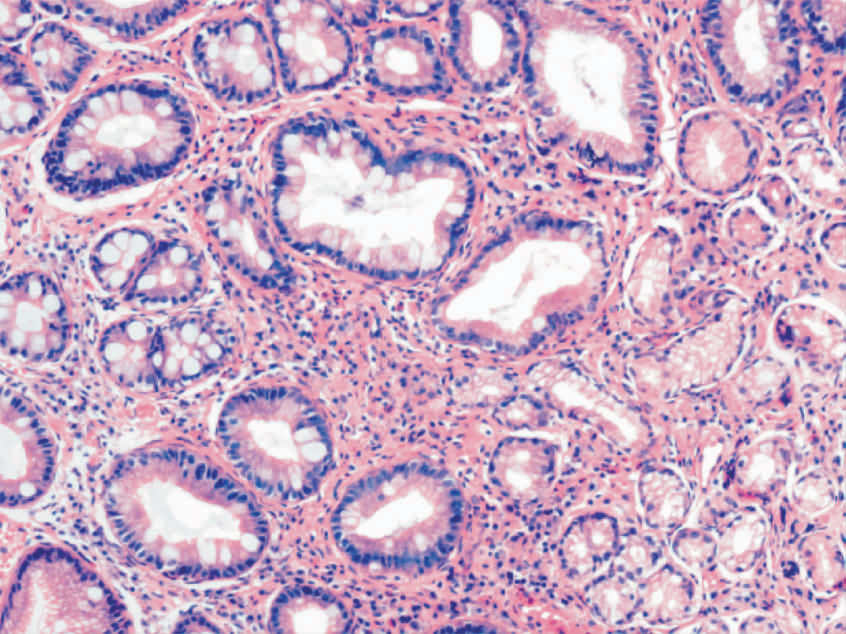
\includegraphics{./images/Image00126.jpg}
 \captionsetup{justification=centering}
 \caption{慢性萎缩性胃炎(HE染色,低倍)}
 \label{fig8-1}
  \end{figure} 

{固有腺体减少伴肠上皮化生,慢性炎症细胞浸润}

\subsubsection{慢性肥厚性胃炎}

慢性肥厚性胃炎少见,病变特点主要为黏膜增厚,皱襞粗大,病变常发生在胃底及胃体部。镜下观,黏膜腺体肥大伴慢性炎症细胞(淋巴细胞、浆细胞为主)浸润。

\subsubsection{疣状胃炎}

病因不明,病变多位于胃窦部,胃黏膜出现许多中心凹陷的疣状突起病灶,镜下病灶中心凹陷部胃黏膜上皮变性坏死并脱落,伴有急性炎性渗出物。

\section{消化性溃疡}

消化性溃疡(peptic
ulcer)是指发生于胃和十二指肠黏膜的慢性溃疡,多见于成人,因其发生与胃液的自我消化有关,故称为消化性溃疡。其中,十二指肠溃疡占发病率的70%,胃溃疡为25%,胃、十二指肠复合性溃疡(胃和十二指肠同时发生溃疡)为5%左右。

溃疡病是一种常见病,呈慢性经过。男性患者多于女性,且多为青壮年,80%的患者年龄在40岁以下。溃疡病的主要临床表现为有规律的上腹部疼痛、反酸、嗳气等。

\subsection{病因与发病机制}

溃疡病的发生是对胃黏膜的损害因素和与防卫因素之间的失衡。可能与幽门螺杆菌的感染、胃酸及胃蛋白酶对自身胃(肠)壁组织消化等因素有关。

\subsubsection{幽门螺杆菌的感染}

幽门螺杆菌感染在溃疡病发病机制中有重要的作用。幽门螺杆菌可分泌尿素酶、裂解蛋白酶、磷酸酯酶等,有利于胃酸直接接触上皮细胞并进入黏膜。

\subsubsection{胃黏膜屏障作用的减弱和破坏}

覆盖在黏膜表面的呈弱碱性的黏液、黏膜上皮顶部的紧密连接、黏膜上皮细胞高度的更新能力以及前列腺素、表皮生长因子的释放是重要屏障。各种原因如胃酸过多、胆汁反流、炎性介质、长期服用某些非甾体类药物、吸烟等,造成胃黏膜屏障作用的破坏。胃酸及胃蛋白酶对自身胃(肠)壁组织的消化是形成溃疡的重要原因。

\subsubsection{神经、内分泌功能的失调}

精神过度紧张或忧虑及迷走神经兴奋可使胃泌素分泌增加,导致胃酸分泌过多,促进溃疡的形成。

\subsubsection{遗传因素}

遗传因素如O型血的人发病率高于一般人群。

\subsection{病理变化}

肉眼观,胃溃疡多位于胃窦部,通常为单个,外形规则呈圆形或椭圆形,直径一般小于2
cm,较深,可达肌层甚至浆膜层。溃疡边缘较整齐,黏膜皱襞呈放射状,底部较平坦干净(图\ref{fig8-2})。

\begin{figure}[!htbp]
 \centering
 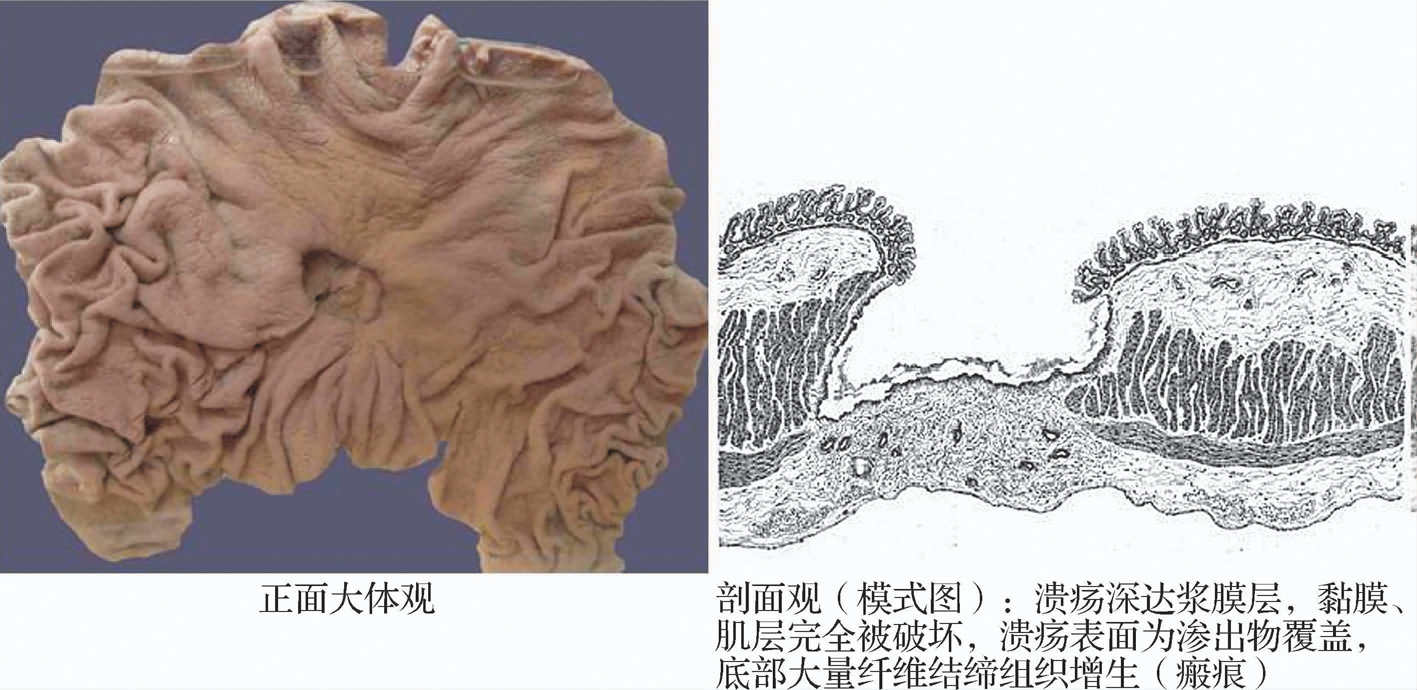
\includegraphics{./images/Image00127.jpg}
 \captionsetup{justification=centering}
 \caption{胃溃疡}
 \label{fig8-2}
  \end{figure} 

十二指肠溃疡常见于十二指肠球部的前壁或后壁。溃疡的特点与胃溃疡相似,只是直径较小,一般为0.5~1
cm,深度较浅,常可多发。

镜下观,溃疡面由浅及深由四层结构组成:最表面为渗出层,由纤维素及各种炎细胞组成。其下方为受胃液腐蚀而形成的坏死组织层。坏死的深部为新鲜的肉芽组织层。溃疡的最深部是随病程延长而逐渐由肉芽组织老化形成的纤维瘢痕层(图\ref{fig8-3})。瘢痕层内常见由于增殖性动脉内膜炎而形成的小动脉管壁增厚、管腔狭窄现象,甚至可见有血栓的形成。小血管的这些改变虽然可以防止因盐酸的侵蚀而导致的血管破裂,起到一定程度的防御作用,但也因其影响了溃疡底部的血供,使溃疡不易愈合。此外,溃疡底部还常可见到损伤的神经纤维断端呈小球状增生,增生的神经末梢对刺激特别敏感,使患者产生疼痛的感觉。

\begin{figure}[!htbp]
 \centering
 
\includegraphics{./images/Image00128.jpg}
 \captionsetup{justification=centering}
 \caption{溃疡底镜下观(HE染色,低倍)}
 \label{fig8-3}
  \end{figure} 

{可见到炎性渗出层(a)、坏死层(b)、肉芽组织层(c)}

\subsection{临床病理联系}

\subsubsection{疼痛}

上腹部有规律的较长期的疼痛是溃疡病的主要症状,但也有10%左右的患者从无上腹部疼痛的病史,而是以其并发症为首发临床表现。由于胃溃疡的发病机制是胃黏膜屏障受损,胃液中氢离子逆弥散入胃壁组织而引起组织损伤,加上病人常有迷走神经张力降低,胃蠕动及排空减慢,胃酸及食糜在胃中停留的时间延长,因此,胃溃疡患者的疼痛一般都表现为进食后(0.5~2小时)疼痛,即所谓的“饭后痛”,当胃排空、胃酸停止分泌时疼痛缓解。十二指肠溃疡则不同,十二指肠溃疡患者在饥饿或夜间时,迷走神经兴奋性过高、胃泌素分泌量过多及壁细胞数量过多,因此胃酸分泌过多,甚至无进食时也可有胃酸分泌。因此常表现为空腹时疼痛,所谓“空腹痛”,一旦进食,食糜与胃酸混合,中和、稀释了胃酸的作用,因此患者反而疼痛缓解。

\subsubsection{嗳气、反酸、呕吐}

幽门梗阻时胃排空受阻,胃内食物发酵,常出现嗳气、反酸现象,十二指肠溃疡患者胃酸分泌过多者,反酸现象更明显。溃疡病变高度活动、疼痛明显或伴有幽门梗阻时,常出现恶心、呕吐症状。

\subsection{结局及并发症}

\subsubsection{愈合}

经过有效的内科治疗,病因消除,大多数溃疡病都可痊愈。当组织变性坏死停止,溃疡底部的渗出和坏死物溶解吸收或脱落,肉芽组织增生填补溃疡创面(缺损),周围黏膜上皮再生覆盖于溃疡的表面,溃疡愈合。破坏的肌层一般不能再生而只能由肉芽组织形成的瘢痕组织修复。

\subsubsection{并发症}

\paragraph{出血}
10%~35%的患者可出现出血,由于胃酸对溃疡底部血管的侵蚀,溃疡病的患者可有程度不同的出血现象。少量出血时,大便隐血试验阳性,也可出现大出血,一次出血量甚至可达1
000ml以上,是上消化道大出血的常见原因之一,患者可出现呕血和(或)柏油样黑便。

\paragraph{穿孔}
5%~15%的患者可出现穿孔,溃疡穿破浆膜层时可引起急性穿孔,胃肠内容物进入腹腔引起急性弥漫性腹膜炎。有时溃疡侵及胃壁或肠壁浆膜层时,浆膜表面因炎症反应与周围的器官(大网膜、肝、胰等)发生粘连,溃疡可穿入这些周围器官而不发生急性弥漫性腹膜炎(可伴有局限性腹膜炎),此称“慢性穿孔”或“穿透性溃疡”。慢性穿孔多见于十二指肠后壁的溃疡,且较急性溃疡穿孔多见,临床表现不太明显,临床一般不将其列为并发症范围。

\paragraph{幽门狭窄}
约占3%,消化性溃疡大部分发生于幽门附近。活动性溃疡引起的幽门充血水肿、痉挛和(或)溃疡愈合过程中形成的多量的瘢痕结缔组织的收缩,常使幽门发生变形狭窄,引起梗阻。梗阻时,常可呕吐隔夜食物。

\paragraph{癌变}
少数胃溃疡可有癌变,一般认为不超过1%。十二指肠溃疡几乎不发生癌变。胃溃疡边缘的黏膜上皮和腺体上皮反复破坏、增生,在致癌因子的作用下上皮细胞最终可发生癌变。

\section{炎症性肠病}

炎症性肠病是一类病因和发病机制尚不十分清楚的肠道炎症性疾病,目前认为其发病与一组导致上皮防御功能缺陷的易感基因以及由正常肠腔内菌群驱动的黏膜免疫系统的激活有关。其中两个主要的代表性疾病是:Crohn病和溃疡性结肠炎。因为有许多共同的临床特征,因此统称为炎症性肠病(inflammatory
bowel disease,IBD),任何年龄均可发病。

\subsection{Crohn病}

Crohn病又称肉芽肿性结肠炎,是一种可累及全消化道的非连续性全层性炎症疾病,最常累及部位为回肠末端、结肠和肛周。临床主要表现为腹痛、腹泻、便血、腹部肿块。常见的肠道并发症包括肛周皮肤溃疡、中毒性巨结肠,极少部分病人可发展为大肠癌,但其发生率明显低于溃疡性结肠炎。多数大肠Crohn病患者经内科治疗无效后需要施行手术切除病变肠管。另外还可出现极为罕见的肠道外并发症如眼葡萄膜炎、多动脉炎、关节强直性脊柱炎等。

\subsubsection{病因与发病机制}

目前病因不明,大多数学者认为具有遗传易感性,可能与分枝杆菌或其他细菌感染有关;大肠Crohn病可能不是独立的疾病,而是对包括血管异常在内的一种复杂反应形式。

\subsubsection{病理变化}

大体:病变呈节段性分布(具有放射影像可以证实的“跳跃”区域),好发于右侧结肠,其中大约1/4病例累及直肠。溃疡可呈线状、匍行性且不连续,其间夹杂水肿的黏膜致黏膜面呈鹅卵石样外观,肠壁由于水肿及继发性的纤维化致肠壁增厚、管腔狭窄,重者溃疡可穿透肠壁形成瘘管。溃疡愈合后会形成长的铁轨状瘢痕。肛门病变见于75%病变,表现为慢性肛裂、瘘管和溃疡。

显微镜下:病变节段的病变累及肠壁全层,黏膜形态相对正常,黏膜呈非特异性炎性反应,肠壁淋巴组织增生,形成淋巴小结,黏膜下层水肿,继而纤维组织增生,肠壁各层增厚。溃疡表面见坏死,明显水肿及中性粒细胞浸润,可见肉芽组织形成及淋巴细胞浸润。约半数可见非干酪性结节病样肉芽肿,肉芽肿由巨噬细胞及多核巨细胞构成,但无干酪样坏死。

\subsection{溃疡性结肠炎}

溃疡性结肠炎是一种病因未明的慢性溃疡性炎症性疾病。疾病通常先累及直肠,逐渐向全结肠蔓延,病程一般很长,临床上有腹痛、腹泻、血性黏液便等症状,病情可多次缓解和加重,常伴有营养缺乏和贫血。溃疡性结肠炎患者大肠癌的发生率有所升高(2%~5%)。严重型和暴发型病例可导致中毒性巨结肠和肠穿孔等并发症。

\subsubsection{病因与发病机制}

病因不明,大多数学者认为具有遗传易感性,尽管其遗传的重要性似乎不如Crohn病明显。

\subsubsection{病理变化}

大体:左半结肠发病,通常起始于直肠乙状结肠区域,有些病例局限在直肠,但大多数病例向近端播散,有时可累及整个结肠。急性期,肠管黏膜表面有血液和黏液附着,呈现湿润有光泽的外观,常见瘀点性出血。肠黏膜出现大片坏死,随后形成大小不同的不规则形溃疡,残存黏膜水肿增生形成息肉样外观,成为假息肉,呈广基隆起性略带红色的结节,典型的结节小而多发,有时结节体积很大,临床和放射影像学可能会误诊为癌。后期,肠管纤维化、缩窄、变短,黏膜萎缩,结肠周围脂肪明显增多。

显微镜下:病变比较弥漫,主要位于黏膜层和黏膜下层,急性期为非特异性炎症,黏膜固有层炎症细胞数目增多,隐窝基底部及腺腔内中性粒细胞聚集,隐窝脓肿出现,由于许多陷窝互相融合并向肠腔破溃而形成大小不一、形状不规则的浅表溃疡,后期溃疡开始愈合,有非特异性肉芽组织覆盖,并可出现假息肉,息肉主要也是由肉芽组织组成,混有炎症性和充血性黏膜。后期病变区肠壁有大量纤维组织增生,在反复发作的患者扁平萎缩的肠黏膜中可见有黏膜腺体的异型增生性改变,提示有癌变的可能。

溃疡性结肠炎与Crohn病最大的病理学区别在于有无肉芽肿性病变及好发部位。

\section{消化系统常见恶性肿瘤}

\subsection{食管癌}

食管癌(carcinoma of
esophagus)是由食管黏膜上皮或腺体发生的恶性肿瘤。患者男多于女,发病年龄多在40岁以上。本病在我国华北及河南地区多发,高发区集中在太行山区附近,河南省林州市是主要高发区。

\subsubsection{病因}

\paragraph{生活饮食习惯}
长期饮酒、吸烟及食用过热饮食可能与本病的发生有关。在我国高发区调查发现,当地某些粮食及食品中含有一定量的亚硝胺,其检出率比非高发区高。这些因素都会刺激食管黏膜,长期的刺激会导致食管黏膜损伤和慢性炎症反应。各种长期不愈的食管炎可能是食管癌的癌前病变。Barrett食管是食管腺癌发生的重要因素。

\paragraph{环境因素}
营养缺乏是食管癌高发区较普遍的现象。食管癌高发区地质土壤中缺钼、硒、钴、锰等微量元素可能是引起食管癌的间接原因。钼是硝酸盐还原酶的成分,可降低植物中的硝酸盐的含量。

\paragraph{遗传因素}
食管癌高发区患者具有一定的家族性。

\subsubsection{病理变化}

食管癌好发于三个生理性狭窄部,食管中段最多见,下段次之,上段最少。可分为早期和中晚期两类。

\paragraph{早期癌}
此期临床上尚无明显症状。内镜下病变处黏膜轻度糜烂或轻度增生颗粒状,钡餐检查,食管基本正常或呈管壁轻度局限性僵硬。病变局限,多为原位癌或黏膜内癌,也有一部分病例癌组织可侵犯黏膜下层,但未侵犯肌层,无淋巴结转移。5年存活率在90%以上,预后较好。镜下观,几乎全部为鳞状细胞癌。

\paragraph{中晚期癌}
此期患者已出现临床症状,如进行性吞咽困难等。肉眼形态可分为4型。

(1)髓质型:肿瘤在食管壁内浸润性生长,使食管壁均匀增厚,管腔变窄。切面癌组织为灰白色,质地较软似脑髓组织,表面可形成浅表溃疡。

(2)蕈伞型:肿瘤为卵圆形扁平肿块,如蘑菇状突入食管腔内。此型浸透肌层者较其他类型少见。

(3)溃疡型:肿瘤表面形成溃疡,溃疡外形不整,边缘隆起,底部凹凸不平,深达肌层。

(4)缩窄型:癌组织在食管壁内浸润生长,累及食管全周,形成明显的环形狭窄,近端食管腔明显扩张。

镜下观,组织学上有鳞状细胞癌、腺癌、小细胞癌、腺棘皮癌等类型。其中以鳞状细胞癌最多见,约占食管癌的90%,腺癌次之。食管腺癌几乎都起源于Barrett食管。

\subsubsection{扩散}

\paragraph{直接浸润}
癌组织穿透食管壁直接侵入邻近器官。食管上段癌可侵入喉部、气管和颈部软组织;中段癌多侵入支气管、肺;下段癌常侵入贲门、膈、心包等处。受浸润的器官可发生相应的并发症,如大出血、化脓性炎及脓肿、食管-支气管瘘等。

\paragraph{淋巴道转移}
转移沿食管淋巴引流途径进行。上段癌常转移到颈部及上纵隔淋巴结;中段癌多转移到食管旁及肺门淋巴结;下段癌常转移到食管旁、贲门及腹腔淋巴结。

\paragraph{血道转移}
主要见于晚期患者,转移到肝及肺为最常见。

\subsection{胃癌}

胃癌(carcinoma of
stomach)是消化道最常见的恶性肿瘤之一。在我国不少地区的恶性肿瘤死亡统计中,胃癌居第一或第二位。胃癌好发于胃窦小弯侧,好发年龄为40~60岁,男多于女。

\subsubsection{病因}

\paragraph{饮食和环境因素}
胃癌有一定的地理分布特点。胃癌的发病率可能与生活习惯以及环境因素有关。亚硝基类化合物经动物实验证明可诱发胃癌发生。

\paragraph{幽门螺杆菌感染}
流行病学调查幽门螺杆菌(HP)感染与胃癌的发生有关。HP可增加细胞的增殖活性、癌基因激活及抑癌基因的失活,诱发胃黏膜上皮细胞的癌变。

另外某些久治不愈的病变慢性萎缩性胃炎、胃溃疡伴有腺上皮异型增生是胃癌发生的病理基础。

\subsubsection{病理变化}

好发部位为胃窦部,特别是小弯侧(约占75%),胃体部则少见,个别地区有特殊的好发部位。

根据胃癌的病理变化进展程度分为早期胃癌与进展期(晚期)胃癌两大类。

\paragraph{早期胃癌}
癌组织浸润仅限于黏膜层及黏膜下层者,无论有无淋巴结转移均属早期胃癌(early
gastric
carcinoma)。早期胃癌经手术切除治疗,预后颇为良好,术后5年生存率达90%以上,10年生存率75%。由于纤维胃镜活检和脱落细胞学检查方法的推广应用,早期胃癌的发现率有了明显提高。

早期胃癌的肉眼形态可分为3种类型:①隆起型(protruded
type,Ⅰ型):肿瘤从胃黏膜表面显著隆起,有时呈息肉状。②表浅型(superficial
type,Ⅱ型):肿瘤表面较平坦,隆起不显著。此型又可细分为:表浅隆起型(superficial
elevated type,Ⅱa型),表浅平坦型(superficial flat
type,Ⅱb型),表浅凹陷型(superficial depressed
type,Ⅱc型),又名癌性糜烂。③凹陷型(excavated
type,Ⅲ型):有溃疡形成,溃疡可深达肌层。此型最为多见。

组织学分型:以高分化管状腺癌最多见,其次为乳头状腺癌,未分化型癌最少。

\begin{center}
    \textbf{知识链接}
\end{center}
\chapterabstract{黏膜剥除术是早期胃癌的有效治疗手段之一。近年来开展的黏膜剥除术主要用于治疗胃肠道的癌前病变和早期胃癌,对癌组织未突破黏膜肌的早期胃癌可以在胃镜下进行黏膜剥除,在完整切除病变后(病理证实是早期癌,且边切缘和底切缘阴性)密切随访、观察,大多数病人预后良好。}

\paragraph{进展期胃癌(中晚期胃癌)}
癌组织浸润到黏膜下层以下者均属进展期胃癌(advanced gastric
carcinoma),或称为中晚期胃癌。癌组织浸润越深,预后越差。

肉眼形态可分为3型:①息肉型或蕈伞型(polypoid or fungating
type):癌组织向黏膜表面生长,呈息肉状或蕈伞状,突入胃腔内。②溃疡型(ulcerative
type):部分癌组织坏死脱落,形成溃疡。溃疡一般多呈皿状,有的边缘隆起,如火山口状(图\ref{fig8-4},表\ref{tab8-1})。③浸润型(infiltrating
type):癌组织向胃壁内呈局限或弥漫浸润,与周围正常组织无明显边界。当弥漫浸润时致胃壁增厚、变硬,胃腔缩小,黏膜皱襞大部消失。典型的弥漫浸润型胃癌其胃状似皮革制成的囊袋,因而有“革囊胃”(linitis
plastica)之称(图\ref{fig8-4})。

\begin{figure}[!htbp]
 \centering
 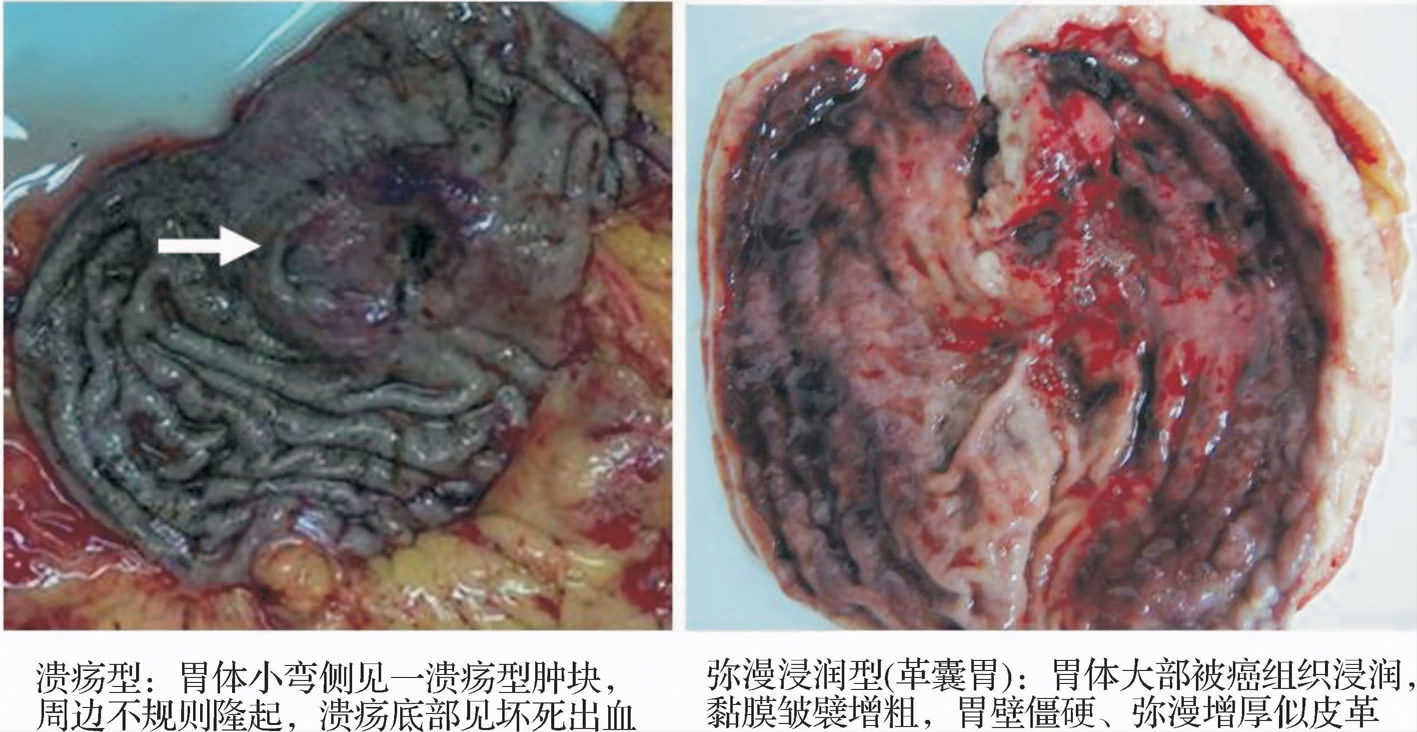
\includegraphics{./images/Image00129.jpg}
 \captionsetup{justification=centering}
 \caption{进展期胃癌大体观}
 \label{fig8-4}
  \end{figure} 

\begin{table}[ht]
    \caption{良、恶性溃疡的肉眼形态区别}
    \label{tab8-1}
    \centering
    \begin{tabular}{lll}
    \toprule
    &良性溃疡&恶性溃疡\\
    \midrule
    外形&圆形或椭圆形&不整齐,皿状或火山口状\\
大小&直径一般<2 cm&直径常>2 cm\\
深度&较深&较浅\\
边缘&整齐,不隆起&不整齐,隆起\\
底部&较平坦&凹凸不平,有坏死出血\\
周围黏膜&皱襞向溃疡集中&皱襞中断,呈结节状肥厚\\
    \bottomrule
    \end{tabular}
\end{table}

镜下观,常见类型有管状腺癌、乳头状腺癌、黏液腺癌和印戒细胞癌等(图\ref{fig8-5})。

\begin{figure}[!htbp]
 \centering
 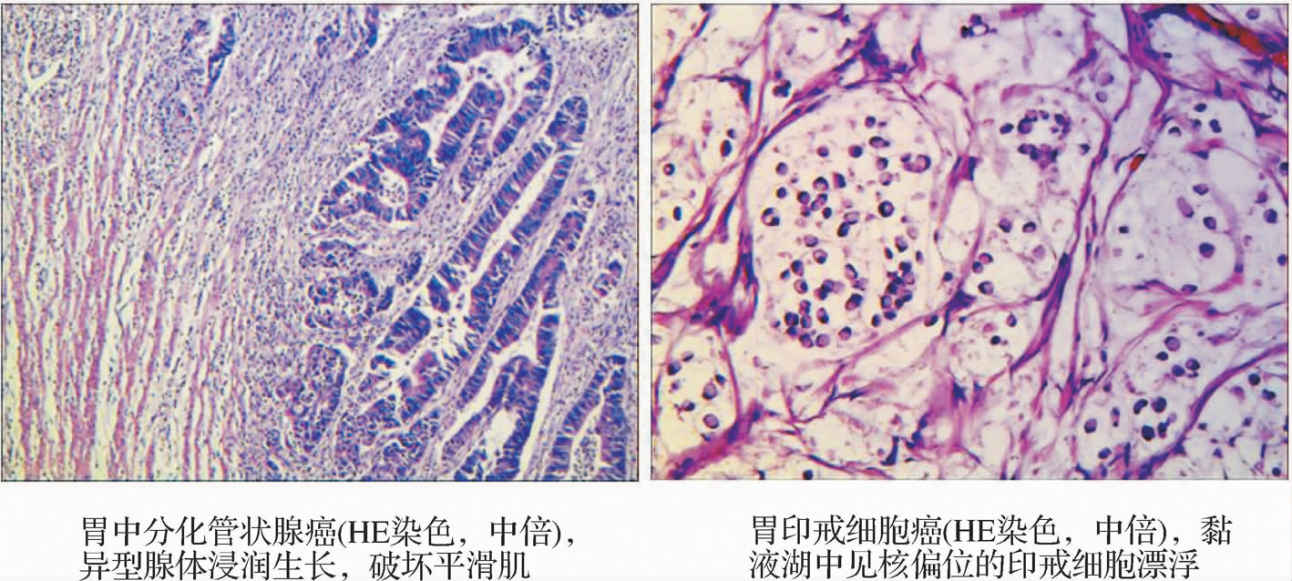
\includegraphics{./images/Image00131.jpg}
 \captionsetup{justification=centering}
 \caption{胃癌组织形态}
 \label{fig8-5}
  \end{figure} 

需要指出,许多胃癌的组织学结构不是单一类型,在同一胃癌标本中往往有两种组织类型同时存在。

\subsubsection{扩散途径}

\paragraph{直接蔓延}
浸润到胃浆膜层的癌组织,可直接扩散至邻近器官和组织,如肝、胰腺及大网膜等。

\paragraph{淋巴道转移}
为胃癌转移的主要途径,以胃小弯侧的胃冠状静脉旁淋巴结及幽门下淋巴结最为多见。可进一步扩散到腹主动脉旁淋巴结、肝门处淋巴结而达肝内;也可到达胰头上方及肠系膜根部淋巴结。转移到胃大弯淋巴结的癌瘤可进一步扩散到大网膜淋巴结。晚期,癌细胞可经胸导管转移到锁骨上淋巴结,且以左锁骨上淋巴结(Virchow信号结)多见。

\paragraph{血道转移}
多在晚期,常经门静脉转移到肝,其次可转移至肺、骨及脑。

\paragraph{种植性转移}
胃癌特别是胃黏液癌细胞浸润至胃浆膜后,可脱落到腹腔,种植于腹壁及盆腔器官腹膜上。有时在卵巢形成转移性黏液癌,称克鲁根勃(Krukenberg)瘤。

\subsection{大肠癌}

大肠癌(carcinoma of large
intestine)亦称结直肠癌,是大肠黏膜上皮和腺体发生的恶性肿瘤。常见于欧美等发达地区。中国是大肠癌的低发地区,但近年由于生活水平提高,饮食结构变化,本癌的发病有上升趋势。患者多为老年人,但中青年人发生率在逐渐上升。患者常有贫血、消瘦,大便次数增多、变形,并有黏液血便。有时出现腹部肿块与肠梗阻症状。

\subsubsection{病因}

\paragraph{饮食因素}
高脂肪低纤维饮食人群中大肠癌的发病率较高。因为高脂肪低纤维食物残渣少不利于形成规律的排便,延长了肠黏膜与食物中含有的致癌物质的接触时间。

\paragraph{遗传因素}
大肠癌的发生有家族高发现象,特别是家族性遗传性多发性息肉病(图\ref{fig8-6})有很高的癌变倾向。

\begin{figure}[!htbp]
 \centering
 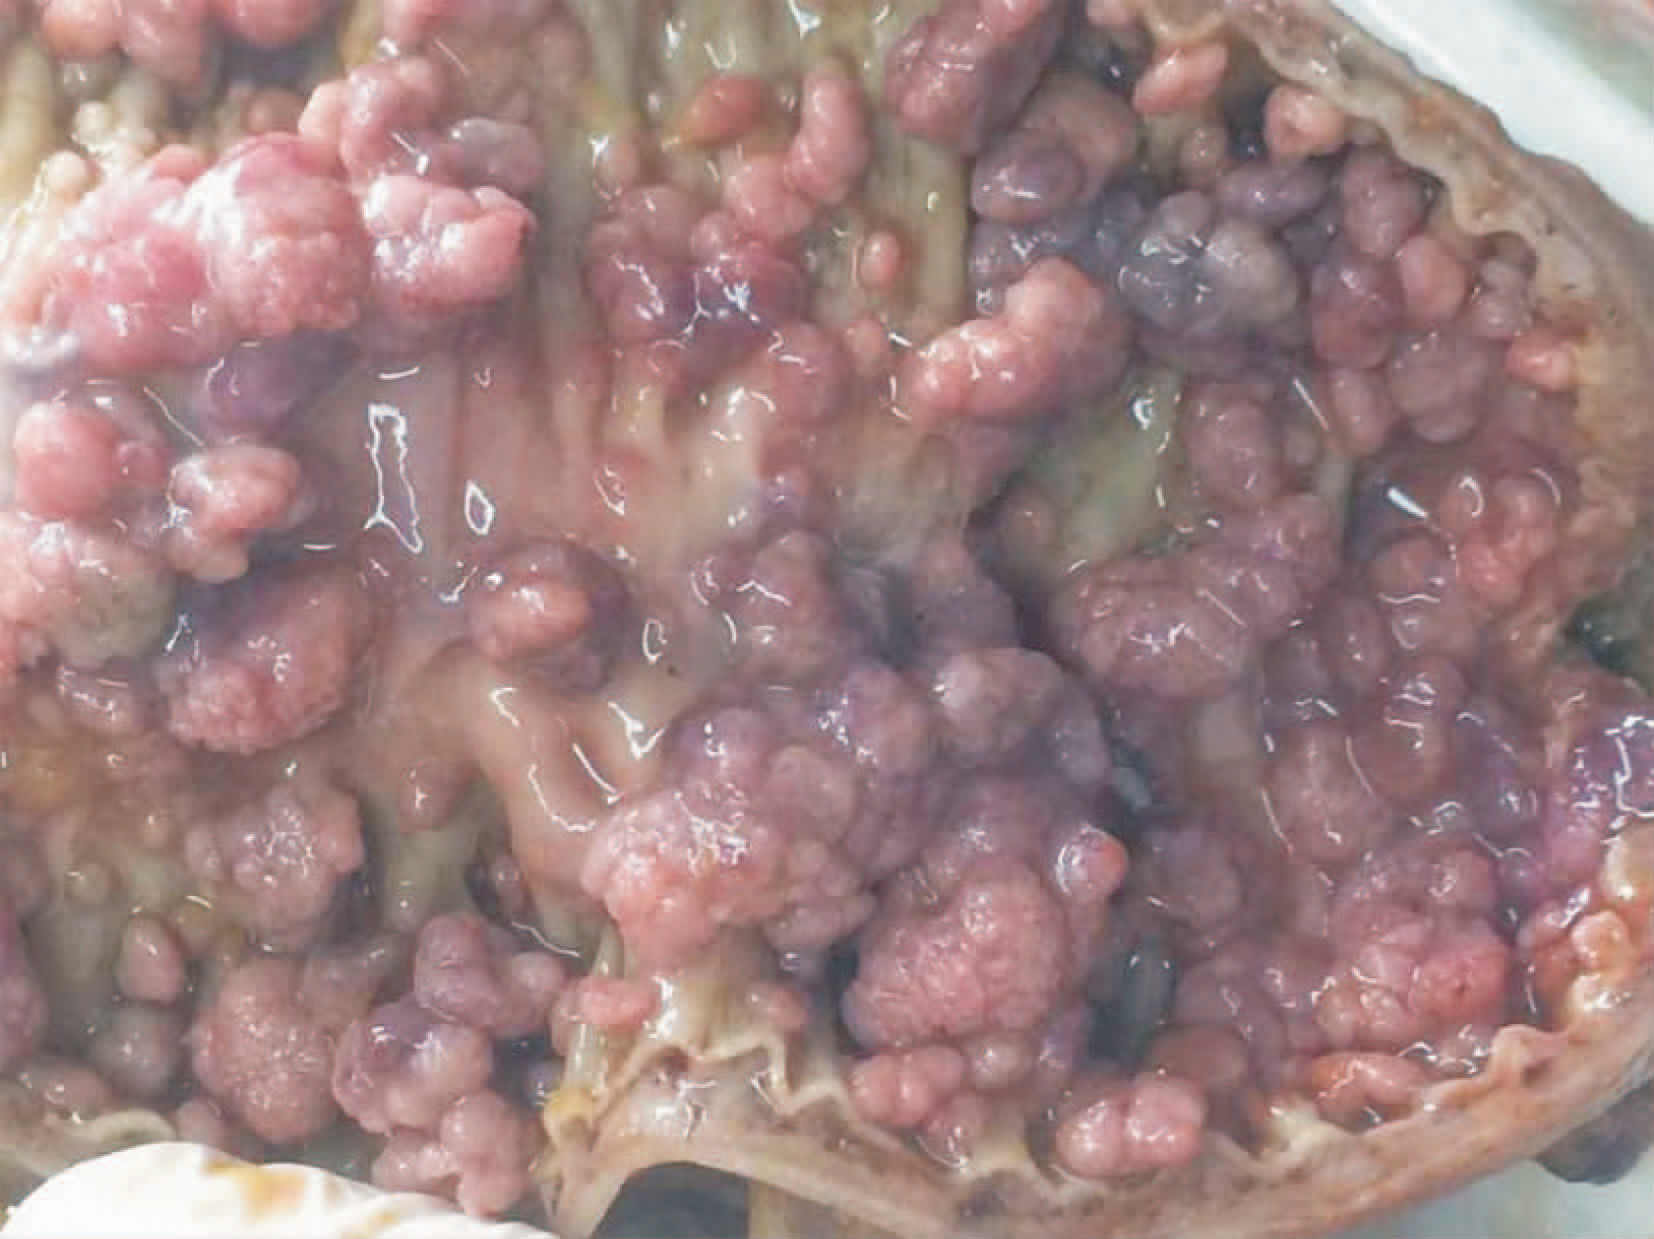
\includegraphics{./images/Image00132.jpg}
 \captionsetup{justification=centering}
 \caption{结肠多发性息肉病}
 \label{fig8-6}
  \end{figure} 

{肠壁黏膜面布满大小不等息肉隆起样腺瘤}

\paragraph{慢性肠疾病}
如息肉样腺瘤、绒毛状腺瘤、慢性血吸虫病、慢性溃疡性结肠炎等由于黏膜上皮过度增生而发展为癌。

\subsubsection{病理变化}

发生部位:大肠癌以直肠为最多,其次为乙状结肠,两者可占全部病例的2/3以上。其次是盲肠、升结肠、降结肠、横结肠。

\paragraph{早期大肠癌}
早期大肠癌是指癌组织仅局限于黏膜及黏膜下层,无淋巴结转移者。

\paragraph{进展期大肠癌}
癌组织浸润到黏膜下层以下者均属进展期大肠癌。肉眼观:一般可分为:隆起型、溃疡型、浸润型、胶样型4型。镜下观组织学类型有:乳头状腺癌、管状腺癌、黏液腺癌、印戒细胞癌、未分化癌、腺鳞癌、鳞状细胞癌。

\subsubsection{分期}

大肠癌的分期对预后有一定的意义,现广泛应用的分期是Dukes改良分期。分期的依据是大肠癌病变在肠壁的扩散范围、是否转移到局部淋巴结以及是否远处转移(表\ref{tab8-2})。

\begin{table}[ht]
    \caption{大肠癌分期及预后}
    \label{tab8-2}
    \centering
    \begin{tabular}{clc}
    \toprule
    分期&肿瘤生长范围&五年存活率(\%)\\
    \midrule
    A&肿瘤限于黏膜层(高级别上皮内瘤变)&100\\
    B$_1$&肿瘤侵及肌层,但未穿透,无淋巴结转移&67\\
    B$_2$&肿瘤穿透肌层,但无淋巴结转移&54\\
    C$_1$&肿瘤未穿透肌层,但淋巴结转移&43\\
    C$_2$&肿瘤穿透全层,并有淋巴结转移&22\\
    D&有远隔脏器转移&极低\\
    \bottomrule
    \end{tabular}
\end{table}

\subsubsection{扩散蔓延}

\paragraph{直接蔓延}
当癌组织已浸润到浆膜层后,可直接蔓延到邻近器官,如前列腺、膀胱、腹膜及腹后壁。

\paragraph{淋巴道转移}
早期肿瘤可沿肠壁神经周围的淋巴间隙扩散,由淋巴管转移到淋巴结。结肠淋巴结可分为结肠上、旁、中间和终末淋巴结4组,结肠癌时均可有转移。直肠癌首先转移到直肠旁淋巴结,以后再扩散,侵入盆腔和肛周组织。

\paragraph{血道转移}
晚期大肠癌可经血行转移到肝、肺、骨等处。肝转移时,转移癌的部位与原发部位有关。一般右侧结肠癌多转移到肝右叶,左侧结肠癌则左、右肝叶均可转移。

\paragraph{种植性转移}
可种植到网膜、直肠子宫窝等处。

\section{病毒性肝炎}

\begin{framed}
{案例8-2}

{【病例摘要】}

患者,男,48岁,因中上腹不适20余天入院。既往自诉体健。20天来无明显诱因下出现中上腹隐痛不适,伴乏力,食欲不振,恶心,呕吐,体重减轻。有乙型肝炎病史15余年。近日于当地医院就诊,查体:心率、呼吸正常,肝性面容,皮肤黄疸,腹部饱满,脾脏肋下一指可触及,叩诊腹部有移动性浊音。腹部CT示腹腔内大量积液,肝脏表面弥漫性高低不平,肝左叶有一占位性病变,大小约4cm×3cm×3cm。

{【问题】}

(1)该患者肝脏病变最有可能的诊断是什么?

(2)试述该患者的疾病是如何发生发展的。
\end{framed}

病毒性肝炎(viral
hepatitis)是由肝炎病毒引起的以肝细胞变性坏死为主要病变的一种常见传染病。肝炎在世界各地都有发病和流行,且发病率有不断升高的趋势。其发病无性别、年龄差异。目前已证实引起病毒性肝炎的肝炎病毒主要有甲(HAV)、乙(HBV)、丙(HCV)、丁(HDV)、戊(HEV)、庚(HGV)6型。在我国以甲型和乙型肝炎为多见。

\subsection{病因与发病机制}

\subsubsection{病因及传播途径}

见表\ref{tab8-3}。

 
\begin{table}[ht]
    \caption{各型肝炎病毒及其相应肝炎的特点}
    \label{tab8-3}
    \centering
    \begin{tabular}{lllp{2cm}p{2cm}l}
    \toprule
    肝炎病毒类型&病毒性质&  潜伏期(周)&传染途径&  转成慢性&暴发型肝炎\\
    \midrule
    HAV & 单链RNA & 2~6 & 肠道 & 无 & 0.1\%~0.4\%\\
HBV & DNA & 4~26 & 密切接触、输血、注射 & 5\% ~10\%&  < 1\%\\
HCV & 单链RNA & 2~26 & 密切接触、输血、注射&  >70\% & 极少\\
HDV & 缺陷性RNA & 4~7 & 密切接触、输血、注射&  共同感染5\%,重叠感染80\%&共同感染3\%~4\%\\
HEV & 单链RNA & 2~8 & 肠道 & 无 & 合并妊娠20\%\\
HGV & 单链RNA & 不详 & 输血、注射 & 无 & 不详\\
    \bottomrule
    \end{tabular}
\end{table}

另外,还有共同感染(coinfection)和重叠感染(super
infection)。前者指HDV与HBV同时感染,后者指在慢性HBV感染的基础上重叠感染HDV。

\subsubsection{发病机制及传播途径}

病毒性肝炎发病过程中肝细胞损伤的发病机制较为复杂,至今尚未完全阐明。造成肝细胞损伤的主要原因是机体对肝炎病毒的免疫反应引起的。

\paragraph{甲型肝炎病毒(HAV)}
通过肠道上皮经门静脉系统到达肝脏,病毒在肝细胞内复制,分泌入胆汁,所以粪便中能检查到病毒。HAV不直接损伤肝细胞,而可能通过细胞免疫机制对肝细胞造成损伤。HAV一般不引起携带者状态,也不导致慢性肝炎。通常起病急,多数可以痊愈,极少发生急性重型肝炎(暴发性肝炎)。

\paragraph{乙型肝炎病毒(HBV)}
完整的HBV颗粒呈球形,具有双层衣壳,是Dane于1970年发现的,故又称Dane颗粒。HBV有一糖蛋白外壳称B型肝炎表面抗原(HBsAg);在感染的肝细胞表面可分泌大量HBsAg,使机体免疫系统,尤其是CD8{+}
T细胞识别并杀伤感染的肝细胞,导致肝细胞坏死或凋亡。在机体缺乏有效的免疫反应的情况下则表现为携带者状态。HBV的核壳体有乙型肝炎核心抗原(HBcAg);在核心区还有一多肽转录物(HBeAg)。HbcAg一直在感染的肝细胞内,而HbeAg则分泌到血液中。在中国,HBV是慢性肝炎的主要致病原,最终导致肝硬化,也可引起急性乙型肝炎、急性重型肝炎和无症状携带者状态。

\paragraph{丙型肝炎病毒(HCV)}
可直接破坏肝细胞,同时免疫机制也是肝细胞损伤的重要原因。HCV感染者约3/4可演变成慢性肝炎。其中20%可进展为肝硬化,部分可发生肝细胞性肝癌。

\paragraph{丁型肝炎病毒(HDV)}
为一复制缺陷性RNA病毒,它必须依赖同HBV复合感染才能复制。其感染可通过两种途径:一种是与HBV同时感染,此类约90%可恢复,仅少数演变为HBV/HDV复合性慢性肝炎,少数发生急性重型肝炎;另外一种是HBV携带者再感染HDV,此类约80%演变为HBV/HDV复合性慢性肝炎,发生急性重型肝炎的比例亦较高。

\paragraph{戊型肝炎病毒(HEV)}
主要通过消化道传播,容易在雨季和洪水过后流行,多见于秋冬季(10~11月)。HEV多感染35岁以上的中老年人,病情往往较重。另外妊娠期戊型肝炎发生重症型肝炎的比例较高。HEV引起的戊型肝炎病毒性肝炎主要见于亚洲和非洲等发展中国家,尤其像印度等国家。HEV一般不导致携带者状态和慢性肝炎。多数预后良好,但在孕妇中死亡率可达20%。

\paragraph{庚型肝炎病毒(HGV)}
透析的患者是易感人群,主要通过血液或者血制品传播,也可经性接触传播。部分患者可变成慢性。此型病毒是否为肝炎病毒尚存争议,目前认为HCV能在单核细胞中复制,因此不一定是嗜肝病毒。

\subsection{基本病变}

各型病毒性肝炎的病变基本相似,都是以肝细胞的变性、坏死为主要特征,同时伴有肝细胞及间质的增生和其他的炎症反应,但变性、坏死、增生的程度不一,其基本病变如下:

\subsubsection{肝细胞变性}

\paragraph{细胞水肿}
为最常见的病变。受损的肝细胞内水分增多,使肝细胞体积增大、胞浆疏松呈网状及染色变浅,称胞浆疏松化。严重时肝细胞形状变圆、胞浆几乎完全透明,整个细胞似吹胀的气球,故称作“气球样变性”。电镜下见内质网不同程度扩张,线粒体明显肿胀,溶酶体增多。

\paragraph{嗜酸性变性(acidophilic degeneration)}
形成原因与气球样变性相反,变性的肝细胞水分脱失、浓缩,体积变小、胞浆嗜酸性增强,故红染。此种变性一般仅累及单个或数个肝细胞。

\subsubsection{肝细胞坏死与凋亡}

\paragraph{溶解性坏死(lytic necrosis)}
最多见。严重的气球样变性最终导致细胞膜破裂,细胞解体,称为“溶解性坏死”。少量的溶解性坏死很快被吸收,因此,病变局部常见不到坏死细胞的痕迹,只见到作为坏死后的炎细胞浸润反应。重型肝炎肝细胞受损严重,肝细胞可不经气球样变性阶段而直接发生大面积的溶解性坏死。不同类型的病毒性肝炎坏死的范围和分布不同,可分为:①点状坏死(spotty
necrosis):指单个或数个肝细胞的坏死,常见于急性普通性肝炎。②碎片状坏死(piecemeal
necrosis):指肝小叶周边部界板肝细胞的灶性坏死和崩解,常见于慢性肝炎。③桥接坏死(bridging
necrosis):指中央静脉与汇管区之间,两个汇管区之间,或两个中央静脉之间出现的互相连接的坏死带,常见于中度与重度慢性肝炎。④大片坏死:指几乎累及整个肝小叶的大范围的肝细胞坏死,常见于重型肝炎。

\paragraph{凋亡}
以往曾被认为是嗜酸性坏死,实质属于细胞凋亡。由嗜酸性变性发展而来,胞质进一步浓缩,核也浓缩消失,最终形成深红色浓染的圆形小体,称为嗜酸性小体(凋亡小体)。凋亡小体形成后很快即可被肝内的枯否氏细胞吞噬消化。

\subsubsection{增生}

\paragraph{肝细胞再生}
坏死的肝细胞由周围的肝细胞通过直接或间接分裂再生而修复。再生的肝细胞体积较大,胞质略呈嗜碱性,细胞核大且深染,有时出现双核甚至三核肝细胞。

\paragraph{间质反应性增生和小胆管增生}
间质反应性增生包括:①枯否氏细胞增生,并可脱入窦腔内变为游走的吞噬细胞,参与炎细胞浸润;②间质细胞和成纤维细胞增生参与损伤的修复。慢性病例在汇管区可见小胆管的增生。

\subsubsection{炎细胞浸润}

肝有炎症时,在汇管区或肝小叶内散在性、灶性炎性细胞浸润,主要是淋巴细胞、单核细胞,有时也可见少量的浆细胞等。

\subsection{临床病理类型}

不同型别的病毒性肝炎,肝细胞变性坏死的范围和程度很不相同,炎症反应的表现也不尽相同,炎症的结局也有较大差异。根据这些不同点,临床上将病毒性肝炎分为急性肝炎、慢性肝炎和重型肝炎。

\subsubsection{急性普通型肝炎}

此型肝炎最为常见。根据患者有无黄疸的出现又分为黄疸型和无黄疸型两种,我国多为无黄疸型,其中以乙型肝炎多见,一部分为丙型。黄疸型肝炎病变稍重,病程较短,多见于甲型、丁型和戊型肝炎。黄疸型和无黄疸型肝炎病理变化基本相同。

病理变化:肉眼观,肝脏肿大,质较软,表面光滑。镜下观,肝细胞广泛变性,以细胞水肿为主,细胞体积增大,呈胞浆疏松化或气球样变性,使肝细胞索排列紊乱、拥挤,肝窦受压变窄。肝细胞坏死现象较轻,可见肝小叶内散在的、范围很小的、仅涉及数个肝细胞的溶解性坏死灶,称点状坏死。也可见到散在的嗜酸性变性或嗜酸性小体形成(图\ref{fig8-7})。肝小叶内与汇管区可见少量炎细胞浸润。黄疸型坏死往往偏重,毛细血管内常有淤胆和胆栓形成。

\begin{figure}[!htbp]
 \centering
 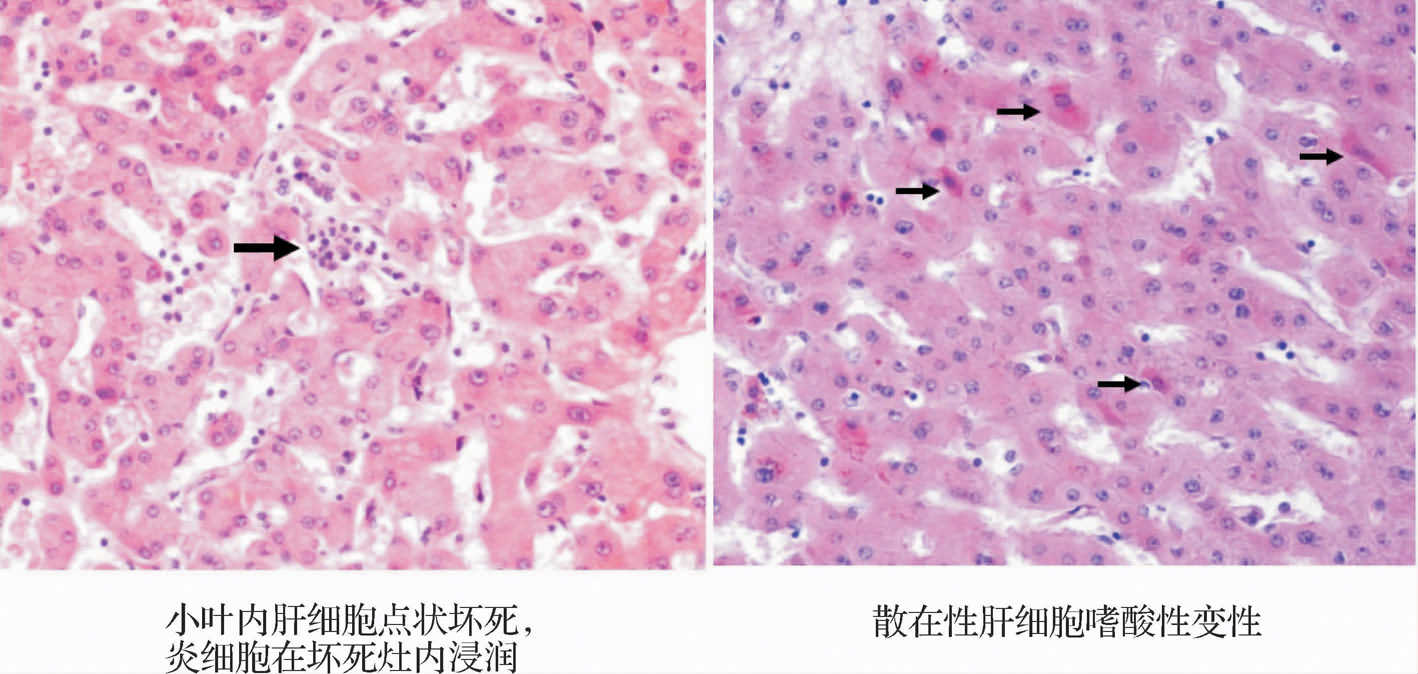
\includegraphics{./images/Image00135.jpg}
 \captionsetup{justification=centering}
 \caption{急性普通型肝炎(HE染色,中倍)}
 \label{fig8-7}
  \end{figure} 

临床病理联系:由于肝细胞弥漫性肿大,使肝体积增大,被膜紧张,为临床上肝大、肝区疼痛或压痛的原因。肝细胞坏死,造成细胞内的酶释放入血,血清丙氨酸氨基转移酶(ALT)升高,同时还可以引起多种肝功能异常,病变严重者出现黄疸。

结局:急性肝炎预后良好,多数患者可在6个月内治愈。由于点状坏死的面积很小,肝内的网状纤维支架在肝细胞发生坏死时保持完整而不发生塌陷,因此,肝细胞可完全再生而修复。部分病人(乙型肝炎5%~10%,丙型肝炎约70%)可转变为慢性肝炎;不到1%的患者可恶化为重型肝炎。

\subsubsection{慢性肝炎}

病毒性肝炎病程持续在半年以上者即为慢性肝炎。导致慢性化的因素有:感染的病原类型、治疗不当、营养不良、同时患有其他传染病、饮酒及服用对肝有损害的药物等,此外,自身免疫反应与慢性肝炎的发生有密切的关系。以往,根据肝内病变不同、临床表现及预后不同,慢性肝炎可分为慢性持续性肝炎和慢性活动性肝炎两种。目前学者们注意到HCV患者由慢性肝炎演变为肝硬化的几率极高,与最初的肝病变程度无关。因而慢性肝炎的病原分型更为重要。现多根据炎症、坏死、纤维化程度,将慢性肝炎分为下述三型:

\paragraph{轻度慢性肝炎}
点状坏死,偶见轻度碎片状坏死。汇管区有较多的淋巴细胞和巨噬细胞浸润,周围有少量纤维组织增生。但肝小叶轮廓清楚,界板无破坏。

\paragraph{中度慢性肝炎}
肝细胞变性、坏死较明显,出现桥接坏死和中度碎片状坏死。小叶内有纤维间隔形成。但小叶结构大部分保存。

\paragraph{重度慢性肝炎}
重度的碎片状坏死和大范围的桥接坏死。坏死区出现肝细胞不规则再生,纤维间隔分割肝小叶结构。

原来分类中的慢性活动性肝炎相当于中、重度慢性肝炎,出现特征性的碎片状坏死和桥接样坏死。晚期逐步转变为肝硬化。

由乙型肝炎病毒引起的慢性肝炎(以及无症状病毒携带者),由于机体抗乙肝病毒免疫力不足或缺乏,不能清除肝内的乙肝病毒和受染肝细胞,因此,肝细胞内的乙肝病毒可以大量复制,使内浆网中出现大量的病毒复制产物HBsAg,HE染色的切片上可见病变肝细胞胞浆内充满均匀红染的细颗粒,使细胞浆呈毛玻璃样改变,这种变性的肝细胞称“毛玻璃样肝细胞”(ground
glass hepatocytes)。

\subsubsection{重型肝炎}

重型肝炎的发病率大约为1%。由于肝组织发生大面积的坏死,肝功能严重受损,常导致急性肝功能不全,死亡率极高。重型肝炎常由乙肝病毒引起,根据起病缓急及病变程度不同,重型肝炎分为急性重型肝炎和亚急性重型肝炎两种。

\paragraph{急性重型肝炎}
很少见,发病率仅为2‰~4‰。本型肝炎起病急,病情凶险,病变发展迅速,病死率极高,如抢救不及时,患者常在两周内死亡,故又名“暴发性肝炎”(fulminant
hepatitis)。

病理变化:肉眼观,肝脏体积明显缩小,重量减轻至600~800
g,尤以左叶为甚。包膜皱缩,质地变软,切面呈红褐色、土黄色或红黄相间的斑纹状,因而又称急性红色肝萎缩或急性黄色肝萎缩。镜下观,肝细胞发生大面积坏死。多数肝小叶全部或大部分发生溶解性坏死,仅在小叶边缘可见少量残留的变性肝细胞。坏死、溶解的肝细胞逐渐被吸收,残存的肝窦明显扩张充血或出血,Kupffer细胞增生肥大,吞噬活跃,整个肝组织呈现一片“荒凉”景象。由于起病急、病变发展迅速、整个病程较短,因此网状纤维支架多无塌陷现象,残存的肝细胞也无明显增生现象。坏死区淋巴细胞、巨噬细胞浸润(图\ref{fig8-8})。

\begin{figure}[!htbp]
 \centering
 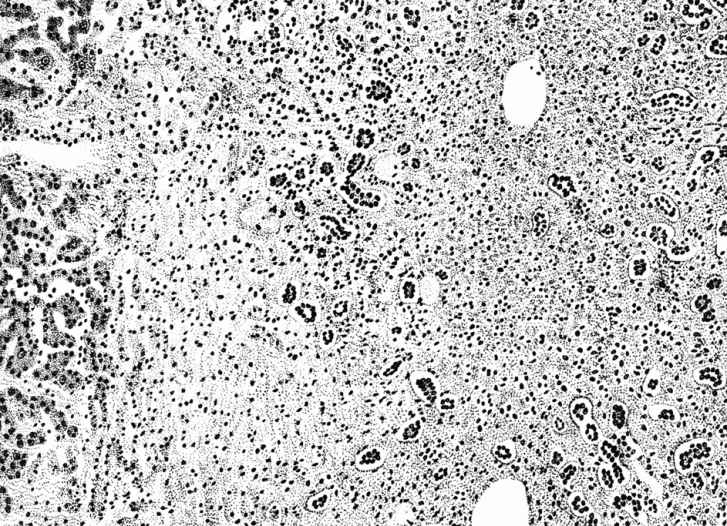
\includegraphics{./images/Image00136.jpg}
 \captionsetup{justification=centering}
 \caption{急性重型肝炎}
 \label{fig8-8}
  \end{figure} 

{肝细胞大块坏死、溶解,仅在汇管区残留少量肝细胞}

结局:本型肝炎大多数在短期内死亡,死亡原因主要为肝功能衰竭(肝性脑病),其次为消化道大出血、肾衰竭、弥散性血管内凝血等。少数迁延为亚急性重型肝炎。

\paragraph{亚急性重型肝炎}
多数由急性重型肝炎迁延而来,少数由急性普通型肝炎恶化进展或一开始就起病较缓,病情发展也较急性重型者慢,病程大约为一至数月。由于肝细胞坏死面积相对较小,残留的肝细胞较多,同时,有肝细胞再生,因此,死亡率较急性重型肝炎低。

病理变化:肉眼观,肝脏体积缩小,表面皱缩不平,切面可因胆汁淤积而呈黄绿色,故又称“亚急性黄色肝萎缩”。病程较长者,肝表面及切面可出现大小不等的浅黄色或黄绿色再生结节,结节周围是灰白色塌陷的坏死区。镜下观,本型肝炎的特点为既有肝细胞的大片坏死,又有肝细胞结节状再生。坏死区的网状纤维支架出现塌陷、融合、胶原化,使再生的肝细胞失去支撑而增生成不规则的肝细胞团,与原肝小叶的结构完全不同,称再生结节。坏死区网状纤维支架塌陷、相邻的汇管区相互靠拢集中,使汇管区扩大,其间可见多量的炎细胞浸润及小胆管、纤维结缔组织增生。

结局:亚急性重型肝炎若治疗及时而病情较轻者,有停止进展和治愈的可能性。若病程迁延时间较长(一年以上),病变可发展为肝硬化。若肝细胞持续变性坏死,病人可死于肝功能衰竭。

临床病理联系:重型肝炎时由于大量肝细胞的迅速溶解坏死,可导致:①胆红素大量入血引起肝细胞性黄疸;②凝血因子合成障碍导致出血倾向;③肝功能衰竭,对各种代谢产物的解毒功能发生障碍。此外,由于胆红素代谢障碍及血循环障碍,还可诱发肾衰竭(称肝肾综合征,hepatorenal
syndrome)。

\section{肝硬化}

肝硬化(liver
cirrhosis)是一种常见的慢性肝脏疾病,引起的因素很多。病变特点为弥漫性的肝细胞变性、坏死以及随之而发生的肝细胞结节状再生和纤维结缔组织增生,导致肝小叶结构和肝内的血管发生了改建,使肝脏变形,质地变硬,故称“肝硬化”。早期肝硬化不出现明显的症状,晚期出现严重的肝功能障碍和门静脉高压症。

\subsection{分类}

由于引起肝硬化的病因及其发病较为复杂,因而至今尚无统一的分类方法。具体如下:

\subsubsection{形态学分类}

\paragraph{小结节性肝硬化}
再生结节直径一般≤3
mm,大小较均匀一致,纤维组织间隔宽度≤2 mm。

\paragraph{大结节性肝硬化}
再生结节直径一般≥3
mm,结节大小不一,最大者可达5~6 cm,纤维组织间隔常较宽,且厚薄不一。

\paragraph{混合结节性肝硬化}
大结节和小结节混合存在,二者比例大致相等。

\paragraph{不全分隔或多小叶性肝硬化}
纤维组织条索状向肝小叶内延伸,但尚未将肝小叶完全分隔,再生结节也不十分明显,或纤维组织包绕多个肝小叶,形成较大的多小叶性结节。此类型属于假小叶尚未完全形成的早期肝硬化或血吸虫病性肝纤维化。

\subsubsection{病因学分类}

按肝硬化的发生原因可分为肝炎性肝硬化(若病毒的感染已消失、无肝炎的表现则称为肝炎后肝硬化)、酒精性肝硬化、胆汁性肝硬化等。

\subsubsection{结合病因及病变的综合分类}

综合分类一般分为门脉性肝硬化、坏死后肝硬化、胆汁性肝硬化、淤血性肝硬化、寄生虫性和色素性肝硬化等。以上除坏死后肝硬化相当于大结节及大小结节混合型外,其余均相当于小结节型。其中门脉性肝硬化最常见,其次为坏死后肝硬化,其他类型较少。

我国常采用结合病因、病变特点以及临床表现的综合分类方法。

\subsection{病因及发病机制}

凡是能持续或反复引起肝实质损害的各种因素,都可以导致肝硬化的发生,其中主要有以下几种:

\subsubsection{病毒性肝炎}

病毒性肝炎是我国肝硬化的主要病因,尤其是乙型和丙型。由病毒性肝炎引起的肝硬化称为肝炎性肝硬化或肝炎后肝硬化。

\subsubsection{慢性酒精中毒}

由于长期酗酒而引起的肝硬化称酒精性肝硬化。酒精性肝硬化是欧美一些国家肝硬化的主要类型(占肝硬化总发病率的40%~50%),我国并不多见,但有上升趋势。长期酗酒者约10%可能发生酒精性肝硬化。乙醇导致肝硬化的原因主要是乙醇对肝细胞能量代谢的干扰以及乙醇的代谢产物(乙醛、乙酸)对肝细胞的直接毒性作用,造成脂肪肝及酒精性肝炎,最终发展成为肝硬化。

\subsubsection{胆道阻塞}

胆石、肿瘤、炎症和畸形等可造成肝内、外胆道阻塞,引起肝内胆汁淤积。由于高浓度的胆酸和胆红素能够直接干扰细胞的氧化磷酸化过程,影响细胞的能量(ATP)产生,因此,肝细胞出现“羽毛状”变性坏死(细胞肿大、胞浆疏松呈网状、核消失)。由胆汁淤积引起的肝硬化称胆汁性肝硬化。

\subsubsection{营养不良}

如食物中长期缺乏蛋氨酸或胆碱类物质时,使肝脏合成磷脂障碍而经过脂肪肝发展为肝硬化。

\subsubsection{其他}

包括长期或过量服用对肝脏有直接毒性的药物或接触某些化学毒物可引起中毒性肝炎、慢性肝淤血晚期,肝细胞因缺氧而发生变性坏死、遗传缺陷引起的代谢紊乱(如肝豆状核变性时的铜沉积于肝脏、血色病时大量含铁血黄素沉积于肝)、寄生虫病引起的肝脏损伤(主要见于慢性血吸虫病)等,最终也可导致肝硬化的发生。

\subsection{病理变化}

肉眼观,肝硬化早、中期体积可正常或稍增大,重量增加,质地正常或稍硬。晚期体积明显缩小,重量减轻,可降至1
000 g以下(甚至达600
g左右),质地变硬。肝脏表面呈结节状,结节可大可小。切面可见再生结节弥漫地分布于整个肝脏,大小与肝表面的结节一致。结节周围为灰白色的纤维间隔包绕(图\ref{fig8-9}a)。

\begin{figure}[!htbp]
 \centering
 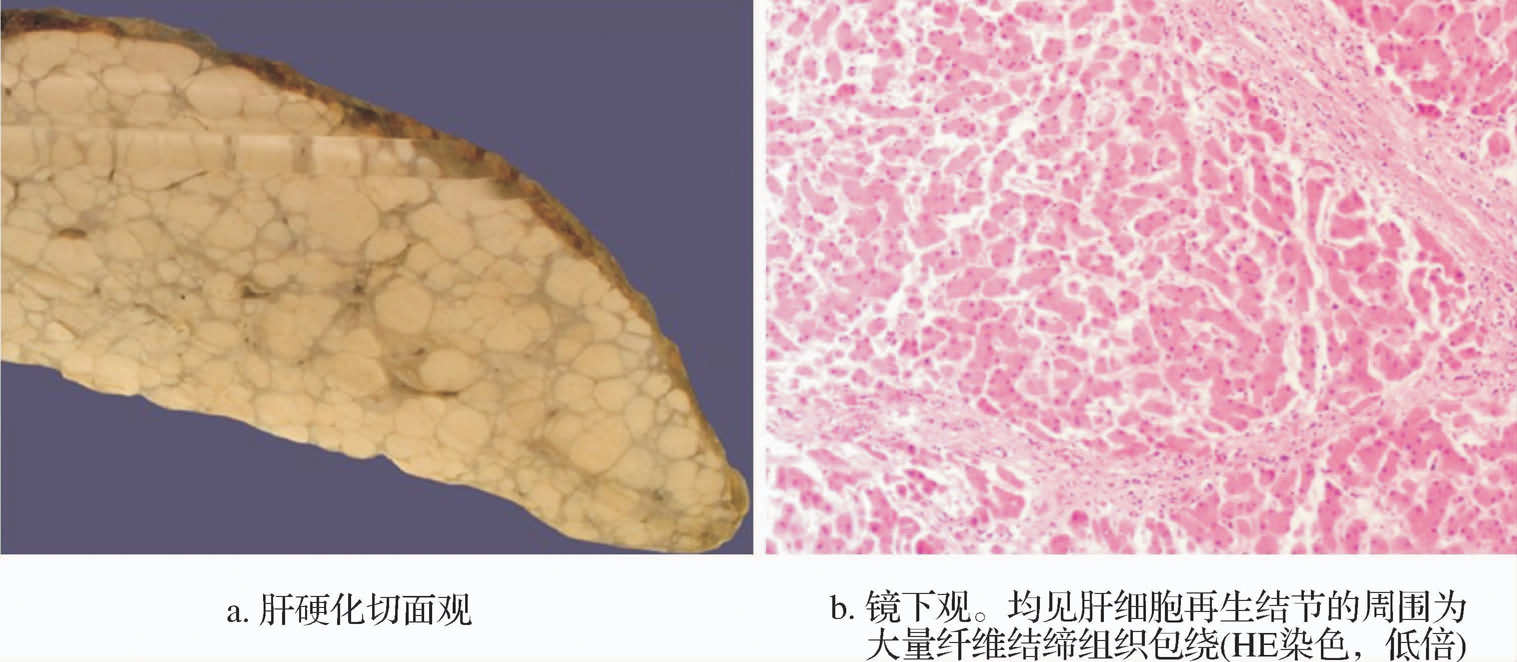
\includegraphics{./images/Image00137.jpg}
 \captionsetup{justification=centering}
 \caption{肝硬化}
 \label{fig8-9}
  \end{figure} 

镜下观,正常肝小叶的结构破坏,增生的纤维组织将肝细胞分割、包绕形成大小不一的肝细胞团,称为假小叶(图\ref{fig8-9}b)。假小叶内肝细胞索排列紊乱,再生结节中的肝细胞常由于病因的持续存在或因缺血而出现不同程度的变性坏死。结节周边再生的肝细胞可表现为细胞体积增大,核深染,出现双核肝细胞。小叶中央静脉偏位或缺如,或有两个以上。甚至可在假小叶内见到汇管区结构。纤维组织增生形成纤维组织间隔,环绕在再生结节的周围,其中常有数量不等的淋巴细胞和巨噬细胞浸润,并有小胆管增生和无明显管腔的假胆管形成。

\subsection{临床病理联系}

\subsubsection{门静脉高压症}

正常人的门静脉压平均为1.76 kPa(18 cmH{2}
O)左右,肝硬化患者门静脉血回流受阻,门静脉压可增高至2.94~4.9
kPa(30~50 cmH{2}
O)以上,并出现一系列的临床征候群,称“门静脉高压症”。

\paragraph{肝硬化门静脉高压症的产生原因}
①假小叶形成及纤维化压迫了小叶下静脉、中央静脉及肝静脉窦,导致门静脉回流受阻。②肝内血管网减少:假小叶形成的过程中,从门静脉到肝静脉的各级血管都有不同程度的破坏,特别是肝窦的数量大量减少;再生结节形成过程中增生的肝细胞团压迫了其周围薄壁的肝静脉小分支;再生结节周围增生的纤维组织的收缩、牵拉常使肝内残留的小血管发生扭曲或闭塞。这些因素使肝内的血管网数目大大减少。③肝动脉和门静脉之间的交通支扩张开放:正常情况下,肝动脉和门静脉之间的交通支不开放,肝硬化形成过程中由于门静脉血回流受阻,肝脏灌流量大大下降,促使肝动脉和门静脉之间的交通支扩张开放,高于门静脉压8~10倍的肝动脉血直接注入压力较低的门静脉分支(图\ref{fig8-10}),这种自身调节功能虽然提高了肝脏的灌注压,部分地改善了再生结节的缺血现象,但也给机体带来了严重的后果。

\begin{figure}[!htbp]
 \centering
 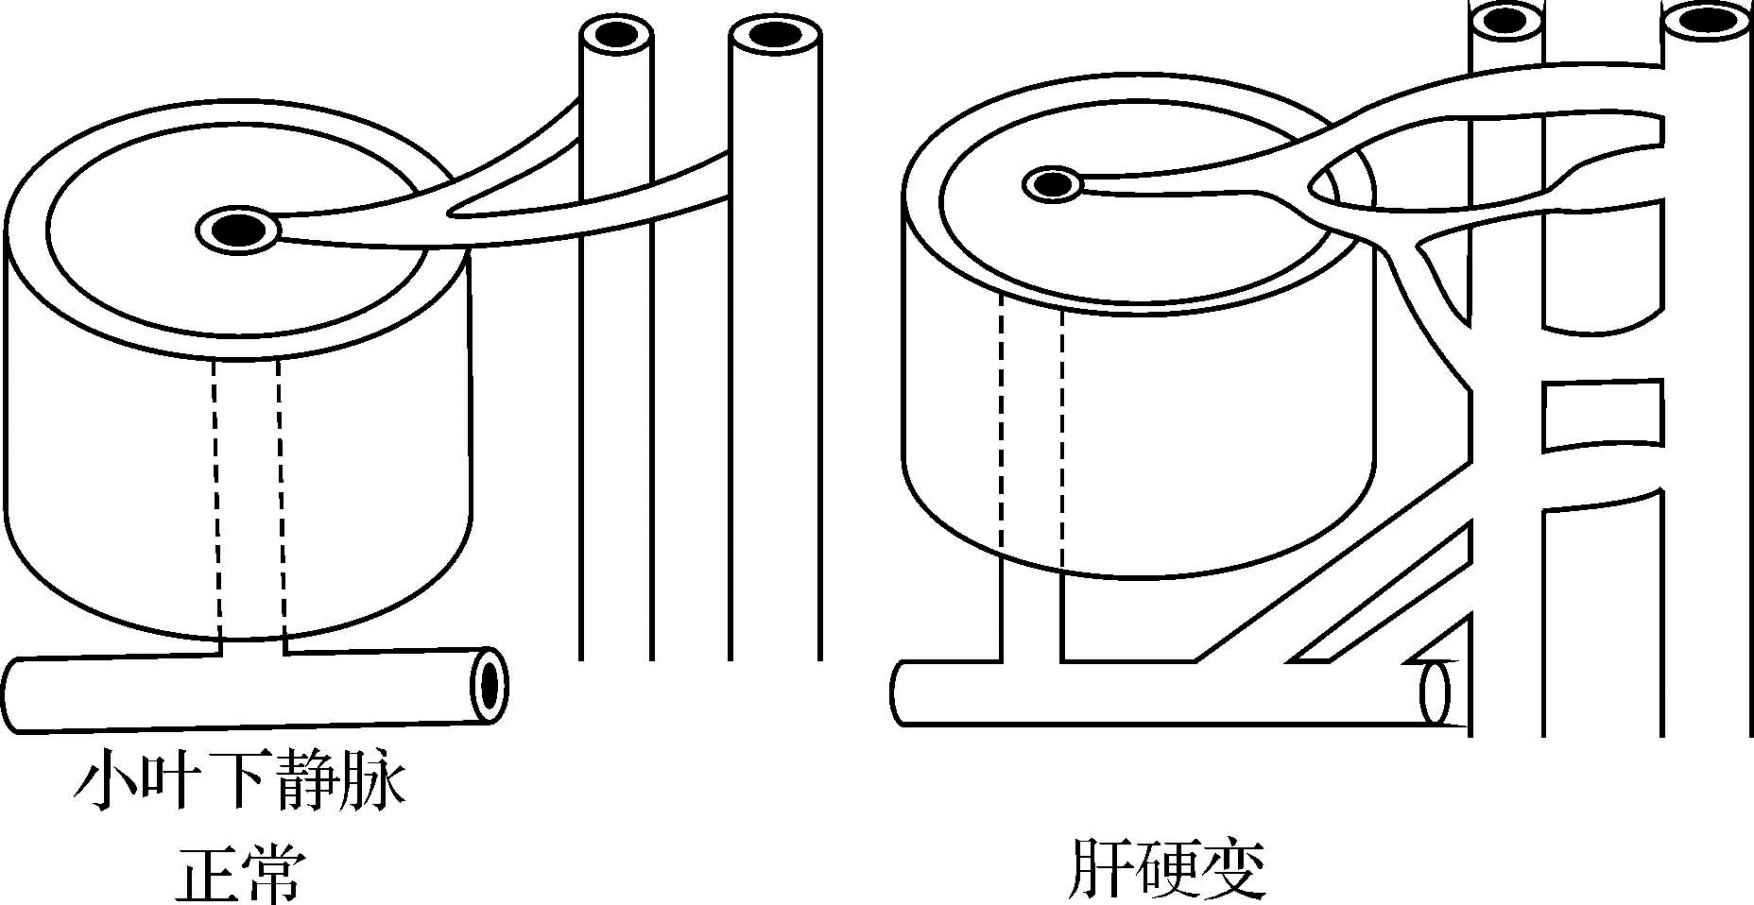
\includegraphics{./images/Image00138.jpg}
 \captionsetup{justification=centering}
 \caption{肝硬化时肝内血管交通支的开放示意}
 \label{fig8-10}
  \end{figure} 

\paragraph{门静脉高压症的临床表现及后果}
(1)慢性淤血性脾脏肿大:肝硬化患者中有70%~85%出现脾肿大。肉眼观:脾脏肿大,重量一般在500
g以下,少数可达800~1 000
g。镜下观:见脾窦扩张,窦内皮增生、肿大,脾小体萎缩,红髓内纤维组织增生,部分可见含铁结节。患者可因脾功能亢进而出现贫血、白细胞及血小板减少症。

(2)腹水:肝硬化晚期,患者腹腔内可积聚大量淡黄色透明的漏出液,称“腹水”。腹水产生的原因是多方面的,主要有:①门静脉高压使门静脉系统的毛细血管流体静压升高,管壁通透性增大,液体漏入腹腔;②肝静脉受再生结节压迫回流受阻,使肝淋巴液生成增多;③肝功能减低,白蛋白合成减少,因低蛋白血症使血浆胶体渗透压降低,也是腹水形成原因;④肝脏灭活激素的功能下降,抗利尿激素、醛固酮灭活不足,导致水钠潴留,促使腹水形成。

(3)侧支循环扩张开放:门静脉压的增高使门静脉与体静脉之间的一些侧支循环血管代偿性扩张开放,部分门静脉血可经这些侧支循环血管由体静脉回流至心脏(图\ref{fig8-11})。主要的侧支循环有:①门静脉血经胃冠状静脉、食管静脉丛、奇静脉入上腔静脉,常致胃底与食管下段静脉丛曲张,甚至破裂发生致命性大出血,这种情况发生在腹压升高或受到粗糙食物磨损时,是肝硬化病人死亡的常见原因之一;②门静脉血经肠系膜下静脉、直肠静脉和髂内静脉进入下腔静脉,引起直肠静脉丛曲张,形成痔疮,破裂可引起便血;③门静脉血经附脐静脉,脐周静脉网,而后向上经胸腹壁静脉进入上腔静脉,向下经腹壁下静脉进入下腔静脉,引起脐周浅静脉高度扩张,形成“海蛇头”(caput
medusae)现象。

\begin{figure}[!htbp]
 \centering
 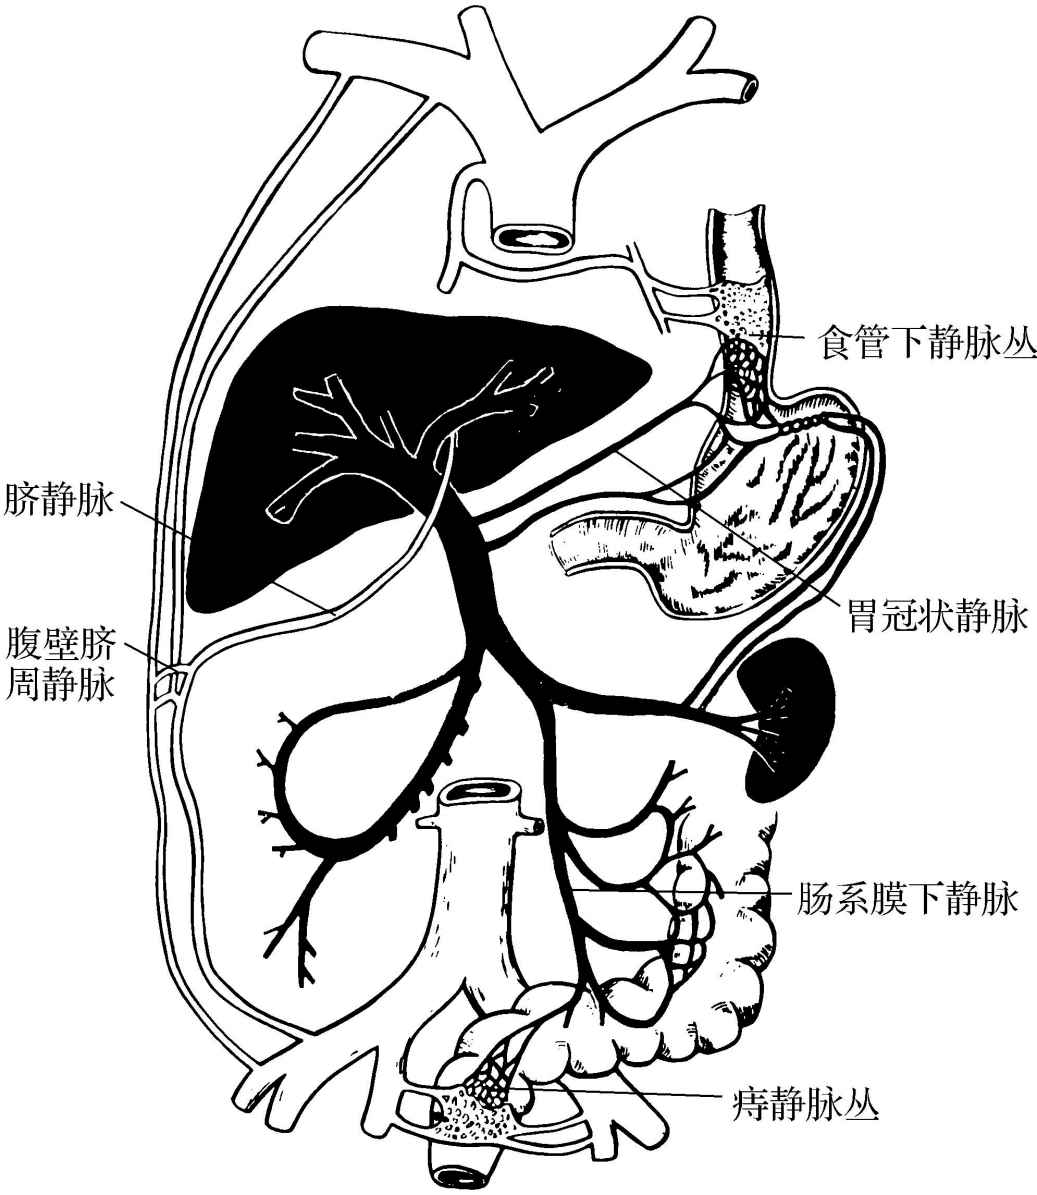
\includegraphics{./images/Image00139.jpg} 
 \captionsetup{justification=centering}
 \caption{肝硬化时侧支循环开放示意图}
 \label{fig8-11}
  \end{figure} 

(4)胃肠道淤血:门静脉压力升高,胃肠道静脉回流受阻,黏膜发生淤血、水肿,消化和吸收功能障碍,患者出现食欲不振、消化不良等症。

{ \subsubsection{肝功能不全} }

\paragraph{激素紊乱}
雌激素灭活不全引起小动脉及其分支发生扩张(蜘蛛状血管痣),男子睾丸萎缩、乳房发育,女子闭经不育。抗利尿激素、醛固酮灭活不全,使尿量减少水钠潴留,促进了腹水和水肿的形成。

\paragraph{出血倾向}
由于凝血酶原、纤维蛋白原等凝血因子合成不足,加上脾功能亢进血小板破坏过多,患者出现鼻衄、齿龈出血、皮肤黏膜出血等。

\paragraph{血浆蛋白合成不足}
白蛋白合成降低,血浆胶体渗透压下降,腹水和水肿不易消退。同时由于从胃肠道吸收的一些抗原物质不经过肝细胞处理,直接经过侧支循环而进入体循环,刺激单核巨噬系统反应性增生,球蛋白合成增多,因此,血浆白蛋白降低且白蛋白、球蛋白比值降低,甚至出现倒置。

\paragraph{解毒功能下降}
胆色素代谢障碍以及肝内胆管受压,患者常有黄疸;机体代谢及肠道吸收来的含氮化合物(特别是氨)不能通过肝脏转化,引起中枢神经系统中毒,患者出现肝性脑病,是肝硬化患者常见的死亡原因之一。

\subsection{结局}

肝硬化早期由于肝细胞有较强的代偿功能,许多肝功能检查正常,但肝形态结构难以恢复正常。晚期肝硬化预后较差,患者常因肝性脑病或上消化道大出血、感染、并发肝癌而死亡。

\section{原发性肝癌}

原发性肝癌(primary carcinoma of
liver)是由肝细胞或肝内胆管上皮细胞发生的恶性肿瘤,简称肝癌。我国发病率较高,属于常见肿瘤之一,多在中年后发病,男多于女。肝癌发病隐匿,早期无临床症状,故临床发现时多已为晚期,死亡率较高。近年来,甲胎蛋白(AFP)测定和影像学检查使早期肝癌的检出率明显提高。一些直径在1
cm以下的早期肝癌被发现并取得满意的疗效。

\subsubsection{病因}

以下因素与肝癌发生有关:

\paragraph{病毒性肝炎}
现知乙型肝炎与肝癌有密切关系,其次为丙型肝炎。肝癌病例HBsAg阳性率可高达80%以上。近年报道,在HBV阳性的肝癌患者可见HBV基因整合到肝癌细胞DNA中。HBV基因组编码的HBx蛋白能够抑制P53蛋白功能,还能激活有丝分裂原活化的蛋白激酶(MAPK)和Janus家族酪氨酸激酶(JAK)信号转导和转录激活因子通路(STATA),活化原癌基因,诱导肝癌发生。HCV的致癌机制尚不明确,HCV在体内不断变异,一些研究发现可能与HCV的直接细胞毒性作用和宿主介导的免疫损伤有关,反复再生的肝细胞可能不断积累细胞的突变,最终发生恶性转化。

\paragraph{肝硬化}
肝硬化与肝癌之间有密切关系。据统计,一般需经7年左右肝硬化可发展为肝癌。

\paragraph{酒精}
是一种肝癌的致癌因子,间接经由肝硬化,而后修补过程中产生肝癌。

\paragraph{真菌及其毒素}
黄曲霉菌、青霉菌、杂色曲霉菌等都可引起实验性肝癌。其中以黄曲霉菌(aspergillus
flavus)最为重要。

\paragraph{亚硝胺类化合物。}
\subsubsection{病理变化}

\paragraph{肉眼类型}
(1)早期肝癌:也称小肝癌,是指单个瘤结节直径在3
cm以下或结节数目不超过2个,直径之和小于3
cm,患者常无症状,而血清AFP阳性的原发性肝癌。形态特点:瘤结节呈球形或分叶状,灰白色质较软,切面无出血坏死,与周围组织界限清楚。(2)中晚期肝癌:肝脏体积明显增大,重量显著增加,可达2
000~3 000
g以上。癌组织可局限于肝的一叶(多为右叶),也可弥散于全肝并大多合并肝硬化。肉眼可分三型:①巨块型:肿瘤体积巨大,甚至达儿头大,圆形,右叶多见。切面中心常有出血、坏死。瘤体周围常有多少不一的卫星状癌结节。本型不合并或仅合并轻度肝硬化。②多结节型:最常见,通常合并有肝硬化。癌结节散在,圆形或椭圆形,大小不等,如融合则形成较大结节。③弥漫型:癌组织弥散于肝内,结节不明显,常发生在肝硬化基础上,形态上与肝硬化易混淆,此型较少见。

\paragraph{组织学类型}
按组织发生可将肝癌分为三大类:(1)肝细胞癌:最多见,是由肝细胞发生的肝癌。其分化较高者癌细胞类似肝细胞,分泌胆汁,癌细胞排列呈巢状,血管多,间质少。分化低者癌细胞异型性明显,常有巨核及多核瘤细胞。有的癌细胞排列成条索状(索状型);亦可呈腺管样(假腺管型)或实体团块状(实体型)。(2)胆管上皮癌:较为少见,是由肝内胆管上皮发生的癌。其组织结构多为腺癌或单纯癌,可分泌黏液,间质较多。较少合并肝硬化。有时继发于华支睾吸虫病。(3)混合性肝癌:具有肝细胞癌及胆管上皮癌两种结构,最少见。

\subsubsection{蔓延和转移}

肝癌首先在肝内蔓延和转移。癌细胞常沿门静脉播散,在肝内形成转移癌结节,还可逆行蔓延至肝外门静脉主干,形成较大的癌栓,有时可阻塞管腔引起门静脉高压。

肝外转移常通过淋巴道转移至肝门淋巴结、上腹部淋巴结和腹膜后淋巴结。晚期可通过肝静脉转移到肺、肾上腺、脑及骨等处。有时肝癌细胞可直接种植到腹膜和卵巢表面,形成种植性转移。

\begin{center}
    \textbf{知识链接}
\end{center}
\chapterabstract{肝癌的恶性度很高,三年生存率和五年生存率较低,特别是中晚期肝癌。近年来随着治疗手段的多样化,生存时间有所延长。介入治疗和肝移植是中晚期肝癌治疗的重要手段。}

\section*{复习与思考}

{一、名词解释}

嗜酸性小体 碎片状坏死 桥接坏死 假小叶 假胆管 小肝癌 早期食管癌 早期胃癌 革囊胃

{二、问答题}

1. 慢性萎缩性胃炎的病理改变有哪些?

2. 请叙述溃疡病的好发部位,肉眼及镜下观病变特点。

3.
胃窦部发现一个溃疡,用学过的病理知识怎样说明此溃疡是良性溃疡还是恶性溃疡?

4. 消化性溃疡有哪些常见的并发症?

5. 病毒性肝炎的基本病变有哪些?

6. 病毒性肝炎的病理类型有哪些?各有何特点?

7. 肝硬化时再生结节和纤维化是如何形成的?

8. 肝硬化门静脉高压的发生原因及主要临床表现是什么?

9. 肝硬化肝功能不全的发生原因及主要临床表现是什么?

10. 中晚期胃癌、食管癌、肝癌的肉眼类型有哪些?

11. 十二指肠溃疡与胃溃疡比较有何特点?

{三、临床病理分析}

病史摘要:

杭××,男,56岁,患支气管炎多年,五天前咳嗽加重,在当地医院用青、链霉素治疗未见好转。三天前开始腹泻、乏力、发热,一天前因颜面、下肢水肿、少尿、谵妄、昏迷而入院治疗。

入院体检,昏迷,贫血貌,瞳孔对光反射存在。肺部可闻及干性啰音。心音稍低,腹部平坦,肝肋下2
cm,剑突下2.5 cm,有压痛。

化验结果,血常规:白细胞计数15×10{9}
/L,中性粒细胞89%,淋巴细胞10%,单核细胞1%,血小板100×10{9}
/L。肝功能:黄疸指数80 U,门冬氨酸氨基转移酶120 U,丙氨酸氨基转移酶415
U,乳酸脱氢酶650 U,血氨107~164 μmol/L。

患者入院后血压下降,昏迷不断加重,经抢救无效死亡。

尸检所见:

体表:全身皮肤及巩膜黄染,皮肤散在出血点,颜面、下肢水肿。

体腔:胸腔、腹腔、心包腔积液,分别有250 ml,300 ml,150 ml。

心脏:重400 g,右心室肺动脉瓣下2 cm处心肌厚0.5 cm,其他均未见明显异常。

主动脉:主动脉各段均散在黄色条纹,粥样斑块,部分斑块出血、小溃疡形成。

肝:体积明显缩小,重660
g,质软,表面切面红黄相间,镜下观肝细胞大片坏死,仅小叶周边残存少量肝细胞。

肺:两肺体积增大,弹性下降,切面呈海绵状,镜下观肺泡腔扩张,肺泡间隔变窄,部分肺泡间隔断裂。

脑、胰、肾、肾上腺等镜下观毛细血管、小静脉扩张充血,散在小灶出血。

讨论题:

1. 根据本例临床病史及病理解剖检查作出全面诊断,列出诊断依据。

2. 试分析病人可能的死亡原因。